% !TeX program = lualatex
% Using VimTeX, you need to reload the plugin (\lx) after having saved the document in order to use LuaLaTeX (thanks to the line above)

\documentclass[a4paper]{book}

% Expanded on !p snip.rv = get_formatted_date() at !p snip.rv = get_formatted_time().

\usepackage{style}

\title{Algebra \\ Prof. Lachowska Anna}
\author{Arthur Herbette}
\date{Monday 7 September 2026}

\begin{document}
\begin{titlepage}
    \centering
    \vspace*{2cm}
    
    {\large EPFL --- Fall 2026\par}
    \vspace{0.5cm}
    {\small MATH-310\par}
    
    \vspace{2cm}
    \rule{\linewidth}{0.4pt}
    \vspace{0.4cm}
    
    {\huge\bfseries Computer Security and Privacy\par}
    \vspace{0.3cm}
    {\large Prof.\ Thomas Bourgeat\par}
    

    \vspace{0.4cm}
    \rule{\linewidth}{0.4pt}
    
    \vfill
    
    {by Arthur Herbette\par}
    \vspace{0.3cm}
    {\small Lecture notes --- Monday 7 September 2026\par}
    
    \vspace{2cm}
\end{titlepage}
This document was originally created for my own use, but I am sharing it because I believe it may be useful to others for studying and reference purposes. However mistake can happen and there will inevitably be some errors, if you found any, you are more than welcome to send me a message (Arthur Hbe on telegram) or to directly do a PR on the repo 
\begin{center}
	\texttt{\href{https://github.com/Arthur926564/LectureNotes}{https://github.com/Arthur926564/LectureNotes}}
\end{center}

If you think that something is missing or that something is not clear, I will be more than happy to add your modification to this document.\\
$ $\\
Unless otherwise stated, all material in these notes is based on the course content, including the diagrams, explanations, and examples.\\
$ $\\
Note also that these notes were taken during the lecture, but not only; some materials was added later (that's why you may read remarks that sounds like I knew the course before taking it).\\
$ $\\
Finally, thanks a lot to Joachim Favre for his help with the setup and whose style is used in this document.

\newpage


\tableofcontents
\newpage

\section*{Introduction}
\begin{parag}{Overview of the course}
	The goal of the course is to 
	\begin{itemize}
	    \item Understand basic concepts and principles of security design and engineering that will \important{outlast current technology}.
	    \item Learn to \important{model threats} and \important{think critically} about security problems 
			\begin{center}
			    \important{adversarial thinking}
			\end{center}
		\item Get familiar with a number of security mechanisms, learn their purpose and limitations building a \important{toolbox for security engineering}
	\end{itemize}
\end{parag}
\chapter{Introduction}%
\label{cha:Introduction}
\begin{parag}{What is computer security}
    The first question that we'll answer is what are we studying in this course, what is this course about 
	\begin{definition}{Computer Security}
		\important{Properties} of a computer system must hold in the presence of a resourced strategic adversary.
	\end{definition}
\end{parag}
\begin{parag}{What Properties?}
    Traditional properties are such 
	\begin{itemize}
	    \item \important{Confidentiality} --- prevention of unauthorized disclosure of information (e.g. The adversary should not be able to read my bank statement)
	    \item \important{Integrity} --- prevention of unauthorized modification of information (e.g. The adversary should not be able to change my bank balance)
	    \item \important{Availability} --- prevention of unauthorized denial of service (e.g. The adversary should not prevent me accessing my bank account)
	\end{itemize}
	But there is also not-so-traditional (But important properties)
	\begin{itemize}
	    \item Authenticity
	    \item Anonymity
	    \item Isolation
	    \item Non-repudiation
	    \item $\vdots$
	\end{itemize}
\end{parag}

\begin{parag}{The Security policy}
	\begin{definition}{Security policy}
    A high-level description of the \important{security properties} that must hold in the system in relation to \important{assets} and \important{principals}.
    \end{definition}
	\begin{itemize}
	    \item \important{Assets} (objects): anything with value that needs to be protected
	    \item \important{Principals} (subjects): people, computer program, services
	\end{itemize}
\end{parag}
\begin{parag}{The resources strategic adversary}
    Coming back on the definition of computer security, what do we mean by '\textit{resourced strategic adversary}'? To do so we need to define the \important{threat model}
	\begin{definition}{Threat model}
	Describes the \important{resources} available to the \important{adversary} and the adversary's capabilities (observe, influence, corrupt, ...)
	\end{definition}
	\begin{itemize}
	    \item The \important{adversary} is a malicious entity aiming at breaching the security policy
	    \item The \important{adversary} is \important{strategic}: the adversary will choose the \textbf{optimal} way to use her resource to mount an attack that violates the security properties.
	\end{itemize}
	(Threat modelling is a very hard task!)
\end{parag}
Here we have defined a lot of key vocabulary to talk about the adversary but we miss a few and here are those:
\begin{definition}{Threat}
What is the feared event, the goal of the adversary that we don’t want materialized
\end{definition}
For instance 
\begin{center}
    \textit{A hacker wants to retrieve money breaking into the bank’s system\\ A student wants to learn my password by looking over my shoulder}
\end{center}

\begin{definition}{Vulnerability}
Specific weakness that could be exploited by adversaries with interest in a lot of different assets
\end{definition}

For instance 
\begin{center}
    \textit{The banking API is not protected. The password appears in plain text in my screen.}
\end{center}

\begin{definition}{Harm}
The bad thing that happens when the threat materializes
\end{definition}
For instance
\begin{center}
    \textit{The adversary steals money, he blocks access to the bank\ldots}
\end{center}

All together this give if we were to expand the computer security definition 
\begin{center}
    Properties define by a security policy of a computer system must hold in presence of a resource strategic adversary described by the threat model
\end{center}
If the \important{properties} hold within the \important{threat model}, it means that there are no \textbf{Vulnerabilities} that can be exploited to materialize threats and no harms happens.

\section{Basic concepts of security engineering}

\begin{parag}{Securing a system}
    In order to secure a system one needs a \important{security mechanism}
	\begin{definition}{Security mechanism}
	Technical mechanism used to ensure that the security policy is not violated by an adversary within the threat model
	\end{definition}
	This can be build with software (programs) + Hardware + Maths (cryptography) \& distributed systems, people and procedures. Security mechanisms can be engineered!
	\begin{subparag}{Example 1}
	    \textbf{Policy}:ensure the log of transactions is not tampered with by a single employee\\
		\textbf{Mechanism}: encrypt the message before sending
	\end{subparag}
	\begin{center}
		Systems are big! We need security mechanism\textbf{S}
	\end{center}
	Security does not necessarily increase linearly with the number of mechanisms. We could create hundred of walls with locked doors while hiding the key below the entrance carpet.
\end{parag}

\begin{parag}{How do we show systems are secure?}
    Here we can see that there is a big asymmetry between the attacker and the defender. On the attacker case, we only need \important{one way} to violate \important{one} security property (within the threat model). The defender on the other hand need that \important{no adversary strategy} can violate the security policy.\\
	$ $\\
	Therefore one can see that the question '\textit{is this system secure?}' is not enough, the correct question is 
	\begin{center}
	    Is this system secure under \important{this} threat model?
	\end{center}
	A system is said 'secure' if an adversary constrained by a \important{Specific threat model} cannot violate the \important{security policy}.\\
	$ $\\
	Then in order to show that systems are secure we need arguments:
	\begin{definition}{Security argument}
	rigorous argument that the security mechanisms in place are indeed effective in maintaining the security policy (verbal of mathematical).\\
	\begin{center}
	    Subject to the assumptions of the threat model
	\end{center}
	\end{definition}
	For a threat model to be useful, the model must constrain the adversary, otherwise we cannot make a security argument. One could just state: \textit{the adversary know everything and can do anything}.

\end{parag}


\begin{parag}{Security engineering}
    In security engineering we have three steps 
	\begin{enumerate}
	    \item High-level specification
				\begin{itemize}
				    \item Define the architecture of the system (e.g., high level block diagram)
				    \item Define the security policy (principals, assets, security properties)
					\item Define the threat model 
				\end{itemize}
		\item  Security design
			\begin{itemize}
			    \item Select/Design security mechanisms
			    \item State your security argument: which controls maintain which properties?
			\end{itemize}
		\item Secure implementation
			\begin{itemize}
			\item \important{Implement} mechanisms
			\item Ensure they \important{conform} to the design model
			\item Security testing
			\end{itemize}
	\end{enumerate}
	\begin{subparag}{Summary}
	    Security problems always involve an adversary.
		\begin{itemize}
			\item  The adversary is strategic, will take the most damaging approach
			\item The adversary’s capabilities define a threat model
			\item Security mechanisms aim at fulfilling a security policy within a threat model
			\item Showing security implies providing a security argument
		\end{itemize} 
	\end{subparag}
\end{parag}













\chapter{Applied Cryptography}%
\label{cha:Applied Cryptography}

\section{Introduction}
\begin{parag}{Why cryptography matters?}
    A lot of data need to move from one place to another while wanting to stay private (i.e. no one can stole the data during the trip). But not only, even data at rest (e.g. your password in your os) need also to not be accessible by a third party. To ensure this, one need to \important{encrypt} data.
\end{parag}
\begin{parag}{What can we do with cryptography}
    Cryptography is also the building block for:
	\begin{itemize}
	    \item \important{Integrity}: Ensuring data hasn't been tampered with (Hashing/Signatures)
	    \item \important{Authentication}: Verifying identity (Protocols)
		\item But also \important{Anonymity}, etc.
	\end{itemize}
	In this first lecture we will focus on the basics of using cryptography for confidentiality
\end{parag}

\subsection{The Core Problem For Today}
The central problem here is to \important{secure communication over an insecure channel}. We need a way for Alice to send a message to Bob, so that Eve (the adversary) cannot read it even though Eve have access to the channel where the massing is passing. 
\begin{framedremark}
confidentiality for data at rest can be seen as a particular case, where Alice $= $ Bob.
\end{framedremark}

\subsection{The origins of cryptography: the quest for confidentiality}
Before going into cryptography, let us first define what are we trying to ensure 
\begin{definition}{confidentiality : }
information cannot be accessed by unauthorized parties
\end{definition}
\begin{center}
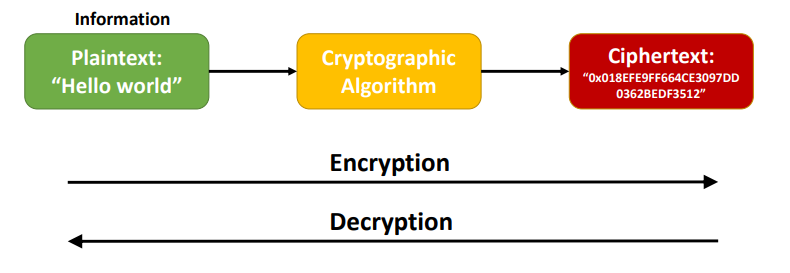
\includegraphics[scale=0.4]{screenshots/2026-10-10.png}
\end{center}
The goal is that the \important{encryption} cannot be reversed without the use of the \important{key}.
\begin{parag}{Cryptography as Functions}
    To have a more formal view of cryptography and being able to ensure confidentiality by proving it mathematically, let us define the encryption/decryption using functions. Here one should define
	\begin{itemize}
	    \item \important{Plaintext} $M$: Original message.
	    \item \important{Key}: $K$ Secret value.
	    \item \important{Ciphertext}: $C$ Scrambled message.
	\end{itemize}
	We then have the following equality 
	\begin{align*} 
		C &= E_K\left(M\right)\\
		M &= D_K\left(C\right)
	\end{align*}
\end{parag}
\begin{parag}{Cryptographic algorithms for confidentiality}
    In order to have confidentiality between Alice and Bob, both needs to either encrypt or decrypt the given message that the other is sending, to do so as seen in the equations above, both Alice and Bob need to share the same key $K$. Having a shared key between Alice and Bob, the algorithm works as follow
	\begin{itemize}
	    \item Encrypt message $m \to \text{Enc}\left(K, M\right)$
	    \item Send encrypted message $\text{Enc}\left(K, M\right) = c$
	    \item Decrypt message $c \to m = \text{Dec}\left(K, c\right)$
	\end{itemize}
	
\end{parag}
\begin{parag}{The core requirement --- Invertibility}
    An statement that we need to make in order to make the encryption/decryption mechanism works is that the decryption function $D_K$ must be the \important{invert} of $E_K$ :
	\begin{align*} 
		\forall K, M, D_K\left(E_K\left(M\right)\right) = M 
	\end{align*}
	If not, Bob cannot recover the original message $M$.
	\begin{framedremark}
	\important{Security requirement}: To provide security, these function must also be \important{hard to invert} without knowing the key $K$. If inverting a given function could be find meaning for instance that if we knew that the function for encryption was $e^{x}$, then it become quite easy to reverse it $\ln\left(c\right) = m$.
	\end{framedremark}
\end{parag}
\begin{parag}{Hard to invert: The Key Space}
    What we mean concretely when saying hard to invert is the following: To find the plaintext $M$, in an ideal cryptosystem, the only viable attack for the adversary (Eve) must be to try every single possible secret key $K$ (a \important{brute force attack})
\end{parag}

\begin{parag}{Example 1: Caesar's Cipher}
    The idea here is simple, we shift every later of the attack by a given number $K$, the key. The algorithm works as follow 
	\begin{itemize}
	    \item \important{Encryption}: Shift each letter by a fixed number $K$
	    \item \important{Decryption}: Shift each letter by a fixed number $-K$
	    \item \important{Key Space}: Only 25 possible keys.
	\end{itemize}
	If for instance the plaintext is \texttt{ATTACK AT DAWN}, the result Ciphertext is \texttt{DWWDFN DW GDZQ}.\\
	$ $\\
	\important{Security Insight}: $\log_2 \left(25\right) \approx 4.6$ bits of security. This is \important{far to small} for real-worls use.
	\begin{framedremark}
	The unit of measure use here $\log_2$ is called the '\textit{bits of security}' which is a logarithmic unit of measurement tat quantifies the \important{amount of computational effort required to break a cryptographic system}. If a system has $n$ bits of security, it means an attacker must perform roughly $2^{n}$ operations (or mathematical steps) to crack it using the best known attack.
	\end{framedremark}
\end{parag}
\begin{parag}{Cryptanalysis: The Flaw}
    \begin{itemize}
        \item Eve knows that Alice wrote a long-enough message for Bob in English.
        \item She knows that English most frequent letter is '\textit{e}'.
        \item She can then simply identify the most frequent letter in the ciphertext: it likely corresponds to the letter '\textit{e}'.
        \item She can then directly recover the key (a number between 0 and 25). This is a \important{frequency analysis attack}.
    \end{itemize}
\end{parag}
\begin{parag}{More than 25 keys: The substitutions Cipher}
	Here you could think, okay then I will just use more letter like $1000$ letters instead of $25$ and then my code is secure. To do so, one can use the substitution Cipher. In this case each letter is mapped to a unique, different letter defined by a \important{permutation} of the 26 letters. What this gives us is a key space of $26! \approx 4.03 \cdot 10^{26}$. $\log_2\left(26!\right) \approx 88.4$ bits of security?\\
	$ $\\
	However this cipher can still easily be broken using the same frequency analysis as before.
\end{parag}
\begin{parag}{Cryptanalysis: The Flaw, Again}
	\begin{itemize}
    	\item The same \important{frequency analysis attack} is effective against the Substitutions Cipher.
    	\item \important{Vulenrability}: The cipher preserves the statistical properties of the plaintext language (e.g., single-letter frequencies).
    	\item If Eve (the attacker) has a long enough ciphertext $C$, statistical analysis will break the cipher, rendering the full $26!$ key space \important{irrelevant}.
    	\item \important{Goal of the adversary}: Notice that the goal of the adversary might not be necessarily to recover the full key depending on the scenario, it might only attempt to recover part of the key (the mapping of a subset of letters) .
    	\item Sometimes the goal of the attacker is even smaller: Eve might want only to know wheter Alice sent the message '\textit{Yes}' or '\textit{No}' to Bob.
	\end{itemize}
\end{parag}

\begin{parag}{Bits of security verus Key Space Size}
    The goal that we would like to reach is that an $N$-bit key should offer security as close to $N$ bits as possible (i.e. require $2^{N}$ attempts). If a 1024-bit key is broken with '\textit{only}' $2^{40}$ attempts (40 bits of security), the algorithm is considered broken. However as seen in the Caesar, having a bigger key is not always a sign better, we also need to take into account that the adversaries are smart.
\end{parag}

\section{Adversaries in Cryptography}
\begin{parag}{Eve's Power: Passive Eavesdropping}
    In Caesar's (and the substitution) Cipher, eve's capabilities were very limited, she was only able to overse a long-enough ciphertext $C$ that corresponds to the encryption of a piece of English (and some compute power to test a few keys). Here this is kind of the lowest possible type of adversaries meaning an adversary with lower rights than this can pretty much do nothing. So let us see other possible adversary models
\end{parag}
\begin{parag}{Other Security Models: Type of Adversaries}
    As seen before, security is a schema that is always measured relative to the power of the \important{adversary (Eve)}
	\begin{itemize}
	    \item \important{Passive Eavesdropper}: Eve can only read the ciphertext
	    \item \important{More Active Attacker}: Eve can somehow influence the system by for example convincing Alice to send to Bob very specific messages, observing the precise time it takes Bob tu run its algorithm, etc... anything that can go beyond just observing the communication.
	\end{itemize}
\end{parag}
\begin{parag}{Active Model 1: Known Plaintext Attack (KPA)}
    The scenario is the following, Eve is given access to multiple pairs $\left(M, C\right)$ corresponding to messages and their corresponding ciphertext, all encrypted with the secret key $K$.\\
	$ $\\
	The goal is to go from this pairs to try to guess the key $K$ in order to decrypt other messages.
	\begin{subparag}{Why is KPA a Realistic Model?}
	    \begin{itemize}
	        \item \important{Standard Headers}: Many encrypted messages contain predictable headers (e.g. '\textit{from:}', or as in the film \textit{The Imitation Game})
	        \item \important{Malicious Guessing}: If Eve guesses a message (or a part of a message) and observes its encryption, she as an $M/C$ pair.
	    \end{itemize}
	\end{subparag}
	\begin{subparag}{KPA and the Substitutions Cipher}
	    If we know take the KPA model trying to attack the substitution cipher, it become even easier to crack it. Imagine that Eve knows that $M =  \text{'THE QUICK BROWN FOX'}$, she immediately recovers the mapping for multiple letters, drastically reducing the effective key space, without even needing to do statistical analysis study.
	\end{subparag}
\end{parag}

\begin{parag}{Active Model 2: Chosen Plaintext Attack (CPA)}
    The scenario is the following: Eve can somehow convince Alice (or the system) to encrypt arbitrary messages (chosen by Eve) with the secret key. More abstractly, for any chosen plaintext $m$, Eve can get access to $E_K\left(m\right)$.
	\begin{framedremark}
	We often say that Eve is assumed to have access to an \important{Encryption Oracle}.
	\end{framedremark}
	\begin{subparag}{Why is CPA a realistic model?}
	    We can imagine two simple scenarios 
		\begin{itemize}
		    \item \important{Alternative Scenario}: Think of a secure messaging service (like Signal  or WhatsApp) that uses the sender's key to encrypt the message. If Eve gets limited access to Alice's phone for a few minuts, she can maybe send any piece of data she choose to Bob, to generate an $\left(M, C\right)$ pair.
		    \item \important{Encryption API}: Eve might interact with an encrypted API endpoint where she provides data and receives the encrypted output.
		\end{itemize}
	\end{subparag}
	\begin{subparag}{CPA and the Substitution Cipher}
	    Here it is easy to show that the substitution cipher is completely broken by CPA as the attacker only have to ask for the encryption of the alphabet.
	\end{subparag}
\end{parag}

\begin{parag}{Practical Threat Model: Side-Channel Attacks}
    The scenario is the following: Eve is allowed to not only access an ideal oracle, but also
measure physical characteristics of the actual implementation while it
is encrypting/decrypting. This allows to have two new attacks:
\begin{itemize}
    \item \textbf{Timing Attack}:  Eve measures how long it takes for a given message to
get encrypted or a ciphertext to be decrypted.
	\item \textbf{Power Analysis}: Eve observes the energy consumed by the device
(e.g., a credit card) doing the crypto.
\end{itemize}

	\begin{subparag}{Why are Side-Channel a Realistic Model?}
	    \begin{itemize}
	        \item \textbf{Malicious Ownership}: ou often own a device (like a phone, smart card, or embedded chip) that holds keys belonging to another principal (e.g., Google, your bank) that are meant to be unreadable to you.
	        \item \textbf{Concrete Example (DRM)}: The decryption key for Digital Rights Management (DRM) content (like a movie or song) is embedded in your media player or console. By measuring power or timing signals, an attacker could potentially extract that secret key.
	    \end{itemize}
	    
	\end{subparag}
\end{parag}






\section{Perfect Secrecy and One-Time-Pad}


\begin{parag}{One-Time-Pad}
    The key is defined as a string $k$ of \important{random} bits \important{as long as the message}. Then one define the encrypted as 
	\begin{align*} 
		\text{Enc}\left(k, m\right) = m \oplus k 
	\end{align*}
	Here we that OTP  is \important{perfectly secure}.
	\begin{itemize}
	    \item For any ciphertext $C$, \important{every possible $M$ is equally likely}
	    \item The key $k$ is uniformly random, so $C$ gives the adversary \important{zero new information} about $M$.
	\end{itemize}
	\begin{definition}{Perfect Secrecy}
	To achieve perfect secrecy for a given encryption algorithm we need the follwing 
	\begin{align*} 
		\forall m, c, P\left(M = m | E_{K}\left(m\right) = c\right) = P\left(M = m\right) 
	\end{align*}
	Which means that for all message and their ciphertext, the probability of a plaintext $M$ being the message knowing the encryption is the same as the probability of the plaintext $M$ being the message.
	\end{definition}
	\begin{theoreme}
	One-Time-Pad achieves perfect secrecy
	\end{theoreme}
	\begin{proof}
	    To do so let us work through the LHS, we use that fact that $m \oplus K =  c \implies K = c \oplus m$ :
		\begin{align*} 
			P\left(M = m | E_K\left(m\right) = c\right) &= \frac{P\left(M = m \cap E_K\left(m\right) = c\right)}{P\left(E_K\left(m\right) = c\right)}  \\
														&= \frac{P\left(M = m \cap \left(m \oplus K\right) = c\right)}{P\left(E_k\left(m\right) = c\right)}\\
														&= \frac{P\left(M = m \cap K = m \oplus c\right)}{P\left(K =  m \oplus c\right)}\\
														&=  \frac{P\left(M = m\right) \cdot  P\left(K =  m \oplus c\right)}{P\left(K = m \oplus c\right)} = P\left(M = m\right)
		\end{align*}
	\end{proof}
	
	
\end{parag}
\begin{parag}{The Key Problem of OTP}
    OTP requires keys that are \important{truly random}, \important{message-length}, and \important{used only once}. And as securely pre-distributing message-length keys for real-world applications is impractical, OTP is not practical for real-world applications.
\end{parag}
\begin{parag}{Cryptanalysis Question: Key Reuse}
    Suppose Alice reuses the key $K$ to encrypt \important{two single-word english message of length 5}, $M_1$ and $M_2$, producing $C_1$ and $C_1$ 
	\begin{align*} 
		C_1 &=  M_1 \oplus K \\
		C_2 = M_2 \oplus K
	\end{align*}
	The goal is to show that even can '\textit{likely}' recover the key and then the two messages $M_1$ and $M_2$. To do so let us multiply our two ciphertexts and use the commutativity of the xor operation 
	\begin{subparag}{Development}
		One can see it as one string $C =  C_1 + C_2$ which is encoded using $K + k$ meaning 
		\begin{align*} 
			C = \left(M_1 + M_2\right) \oplus \left(K + K\right) 
		\end{align*}
		Where $+$ is string concatenation. Here one could seek to show that $P\left(M = m | E_K\left(m\right) = c\right) > P\left(M = m\right)$ 
		\begin{align*} 
			P\left(M = m | E_K\left(m\right) c\right) &= \frac{P\left(M = m \cap E_K\left(m\right) = c\right)}{P\left(E_K\left(m\right) = c\right)} \\
			&= \frac{P\left(M = m \cap \left(m_1 + m_2 \oplus K + K\right) = c_1 + c_2\right)}{P\left(E_K\left(m_1 + m_2\right) =  c_1 + c_2\right)}\\
			&= \frac{P\left(M = m\right) \cdot  P\left(K + K =  m_1 + m_2 \oplus c_1 + c_2\right)}{P\left(K + K = m_1\right)}
		\end{align*}
		However here we have that $K' = K + K$ is not uniformly distributed hence
		Things to fixhere
	\end{subparag}
\end{parag}


\begin{parag}{OTP: Integrity is NOT included}
    OTP guarantees \important{confidentiality} (nobody can read it) however it \textbf{does not} guarantee \important{integrity} (nobody can tamper with it).
	\begin{subparag}{Attack Example (Eve flips the first bit of $M$)}
	    Imagine that Eve flips the first bit of $C$ to get $C'$.\\
		$ $\\
		Bob decrypts $C' : M' = C' \oplus K = \left(M \oplus K \oplus \Delta\right) \oplus K =  M \oplus \Delta$.\\
		$ $\\
		The result is that Eve successfully changed the message ($M'$ is $M$ with one bit flipped) \important{without knowing $K$}
	\end{subparag}

\end{parag}





\section{From OTP to Stream Ciphers}
\begin{parag}{Two Main Types of Symmetric Schemes}
	\begin{definition}{Symmetric Schemes}
	Encryption of plaintext and decryption of ciphertext are done using the \important{same key}
	\end{definition}
	\begin{itemize}
	    \item \important{Block Ciphers}: Operate on fixed-size blocks (e.g., 128 bits).
	    \item \important{Stream Ciphers}: Operate one bit/byte at a time, like a pseudo-OTP. (Example \important{ChaCha20})
	\end{itemize}
	We also need a fixed-size input to symmetric cryptographic primitives, the size of the key influences the level of security provided
	\begin{subparag}{Key properties}
	    \begin{itemize}
	        \item \textbf{Known to both parties}: Partners must agree on the key before starting using the primitive
	        \item \textbf{It is reused}: The key is pre-shared one (key do have a '\textit{duration}') and then reused 
	        \item \textbf{It must be secret}: revealing the key eliminates any protection provided by the primitive
	    \end{itemize}
	\end{subparag}
\end{parag}


\begin{parag}{Stream Ciphers: The pseudo-OTP}
    A stream cipher attempt to emulate the OTP's security while solving the key length problem.
	\begin{itemize}
	    \item \textbf{Short Key} ($k$): Alice and Bob share a small, manageable key
	    \item \textbf{Key stream generator}: Uses $K$ and an \important{initialization vector (IV)} A to produce an arbitrary long, pseudo-random bit stream $S$
	    \item \textbf{Encryption} $C =  M \oplus S$
	\end{itemize}
	Question: Why does the Key Stream Generator takes in also an IV, and not just the key 
	\begin{subparag}{Answer}
	    The KSG needs an IV to make sure that the encryption of two different messages will generate two different randomness, without that, one could simply XOR two ciphertexts together to recover the prefix of S, and decode future messages.
	\end{subparag}
\end{parag}
\begin{parag}{KSG: Finite Secret, Infinite '\textit{Randomness}'?}
	We are generating \important{potentially infinitely long randomness} (the stream $S$) from a \important{finite secret} ($K$). The security here only hold on the fact that $S$ is being computationally indistinguishable from a truly random OTP key.
\begin{center}
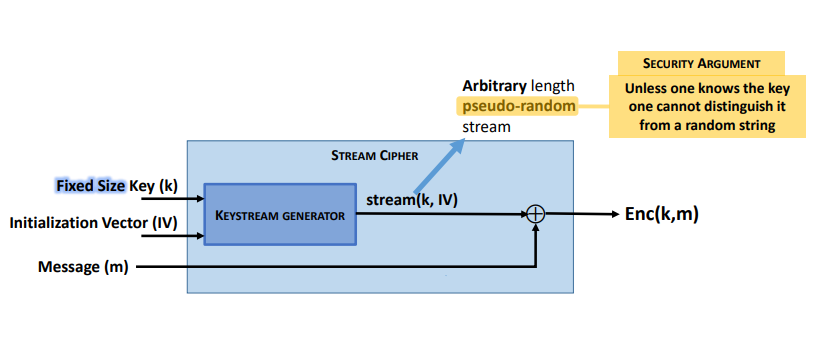
\includegraphics[scale=0.4]{screenshots/2026-10-10_1.png}
\end{center}
\end{parag}
\begin{center}
\begin{tabular}{c|c}
	(+) Speed & Algorithm are linear in time and constant in space.  \\
	\hline
	(+) Low Error Propagation & Errors in one bit do not affect subsequent symbols. \\
	\hline
	(-) Low Diffusion & A change in one plaintext bit only affects one ciphertext bit. \\
	\hline
	(-) Susceptibility to Modification & Low diffusion makes it easier to tamper with the message (like the OTP). \\
\end{tabular}
\end{center}

\begin{parag}{Cryptanalysis: The Problem with Periodicity}
    Key Stream Generators which have finite state are eventually \important{periodic}, hence if the message is longer than the period, the stream repeats which allows attacker to exploit it: if the period is identified, and too small, the key stream is known for the entire message.
\end{parag}



\subsection{Interlude on building KSG}
\begin{framedremark}
You are not expected to fully understand the following subsection, they are here to illustrate some design patterns for KSG, and challenges involved in building secure KSG, and hint at the math needed to study these objects.
\end{framedremark}
\paragraph{The linear Feedback Shift Register Building block for KSG}%
\label{par:The linear Feedback Shift Register Building block for KSG}

\begin{itemize}
    \item  \textbf{Linear Recurrence Relation}, The next output bit is a linear function (XOR) of previous bits, apply a recurrence relation to extend the initial random sequence of bits, into an arbitrary length sequence of (maybe?) randomly looking bits:
    \item For example, start with an initial state of 4 bits, $a_0, \ldots, a_3$ and 
		\begin{align*} 
			a_n =  a_{n-3} \oplus a_{n-4} 
		\end{align*}
		\item Output Sequence (starting from $1, 0, 0, 0$): $1, 0, 0, 0, 1, 0, 0, 1, 1, \ldots$
		\item \textbf{Advantage}: Uses only \textbf{shift registers} (for state storage) and \textbf{XOR gates} (for feedback), so it is extremely fast and efficient to implement in hardware.
\end{itemize}
\begin{parag}{Randomness of LFSR}
    \begin{itemize}
        \item \textbf{Maximal Period}: If the characteristic polynomial (AICC1) of the recurrence relation of the LFSR is primitive (MATH-215, Algebra 3), the maximum possible number of states before repeating: For an L-bit register, the maximum period is $2^{L}-1$ states.
    	\item \textbf{Distribution Property}: As a consequence, the sequence generated exhibit good distribution properties. Specifically, every possible nonzero state appears exactly once in the cycle, so over one full cycle of values, the output sequence are highly balanced. For example, the sequence will contain exactly $2^{L-1}$ ones and $2^{L-1}-1$ zeros. 
    \end{itemize}
\end{parag}
\begin{parag}{LFSR --- Math Danger}
    \begin{itemize}
        \item Despite passing some statistical tests, the underlying operation of an LFSR is purely \textbf{linear}
        \item \textbf{Consequence}: Techniques like the Berlekamp-Massey algorithm (beyond the scope of the class) can recover the entire LFSR state and the key stream by observing only a short segment of the output, breaking the cipher.
        \item \textbf{LFSRs should not be used directly as a Key Stream Generators}, though it has been traditionally used as a building block of Key Stream Generators
    \end{itemize}
\end{parag}

\begin{parag}{The A5/1 Cipher}
    \begin{itemize}
        \item A5/1: Used historically to secure GSM mobile phone communications.
        \item It was built by \textbf{combining multiple LFSRs} in a non-linear way to try and overcome the linearity flaw while still being cheap and having the nice statistical properties.
        \item \textbf{The Break}: despite the increased complexity, mathematical weaknesses were found, allowing the cipher to be broken much fast than brute force.
    \end{itemize}
    \begin{center}
    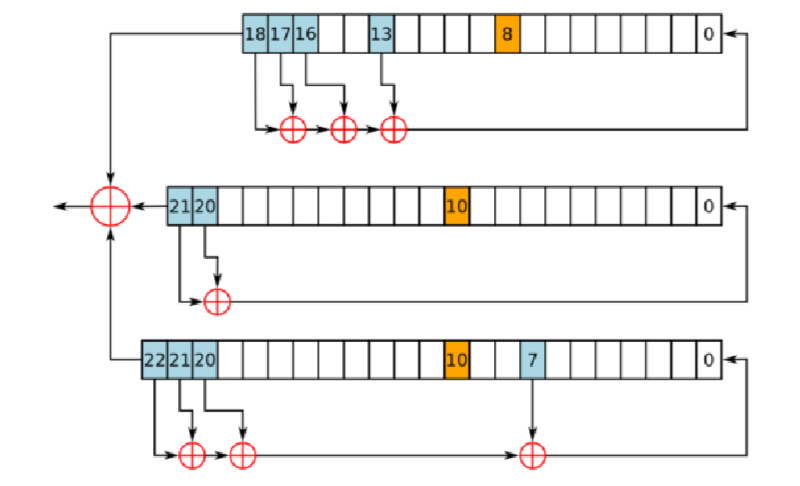
\includegraphics[scale=0.3]{screenshots/2026-10-10_2.png}
    \end{center}
\end{parag}

\begin{parag}{Non borken Stream Ciphers}
    There are alternative, modern stream ciphers for which there are no known practical cryptanalysis. Some example are \important{Trivium} (based on NLFSRs, variation of LFSRs) and \important{Salsa20} (using different techniques).
\end{parag}
\begin{figure}[htpb]
	\centering
	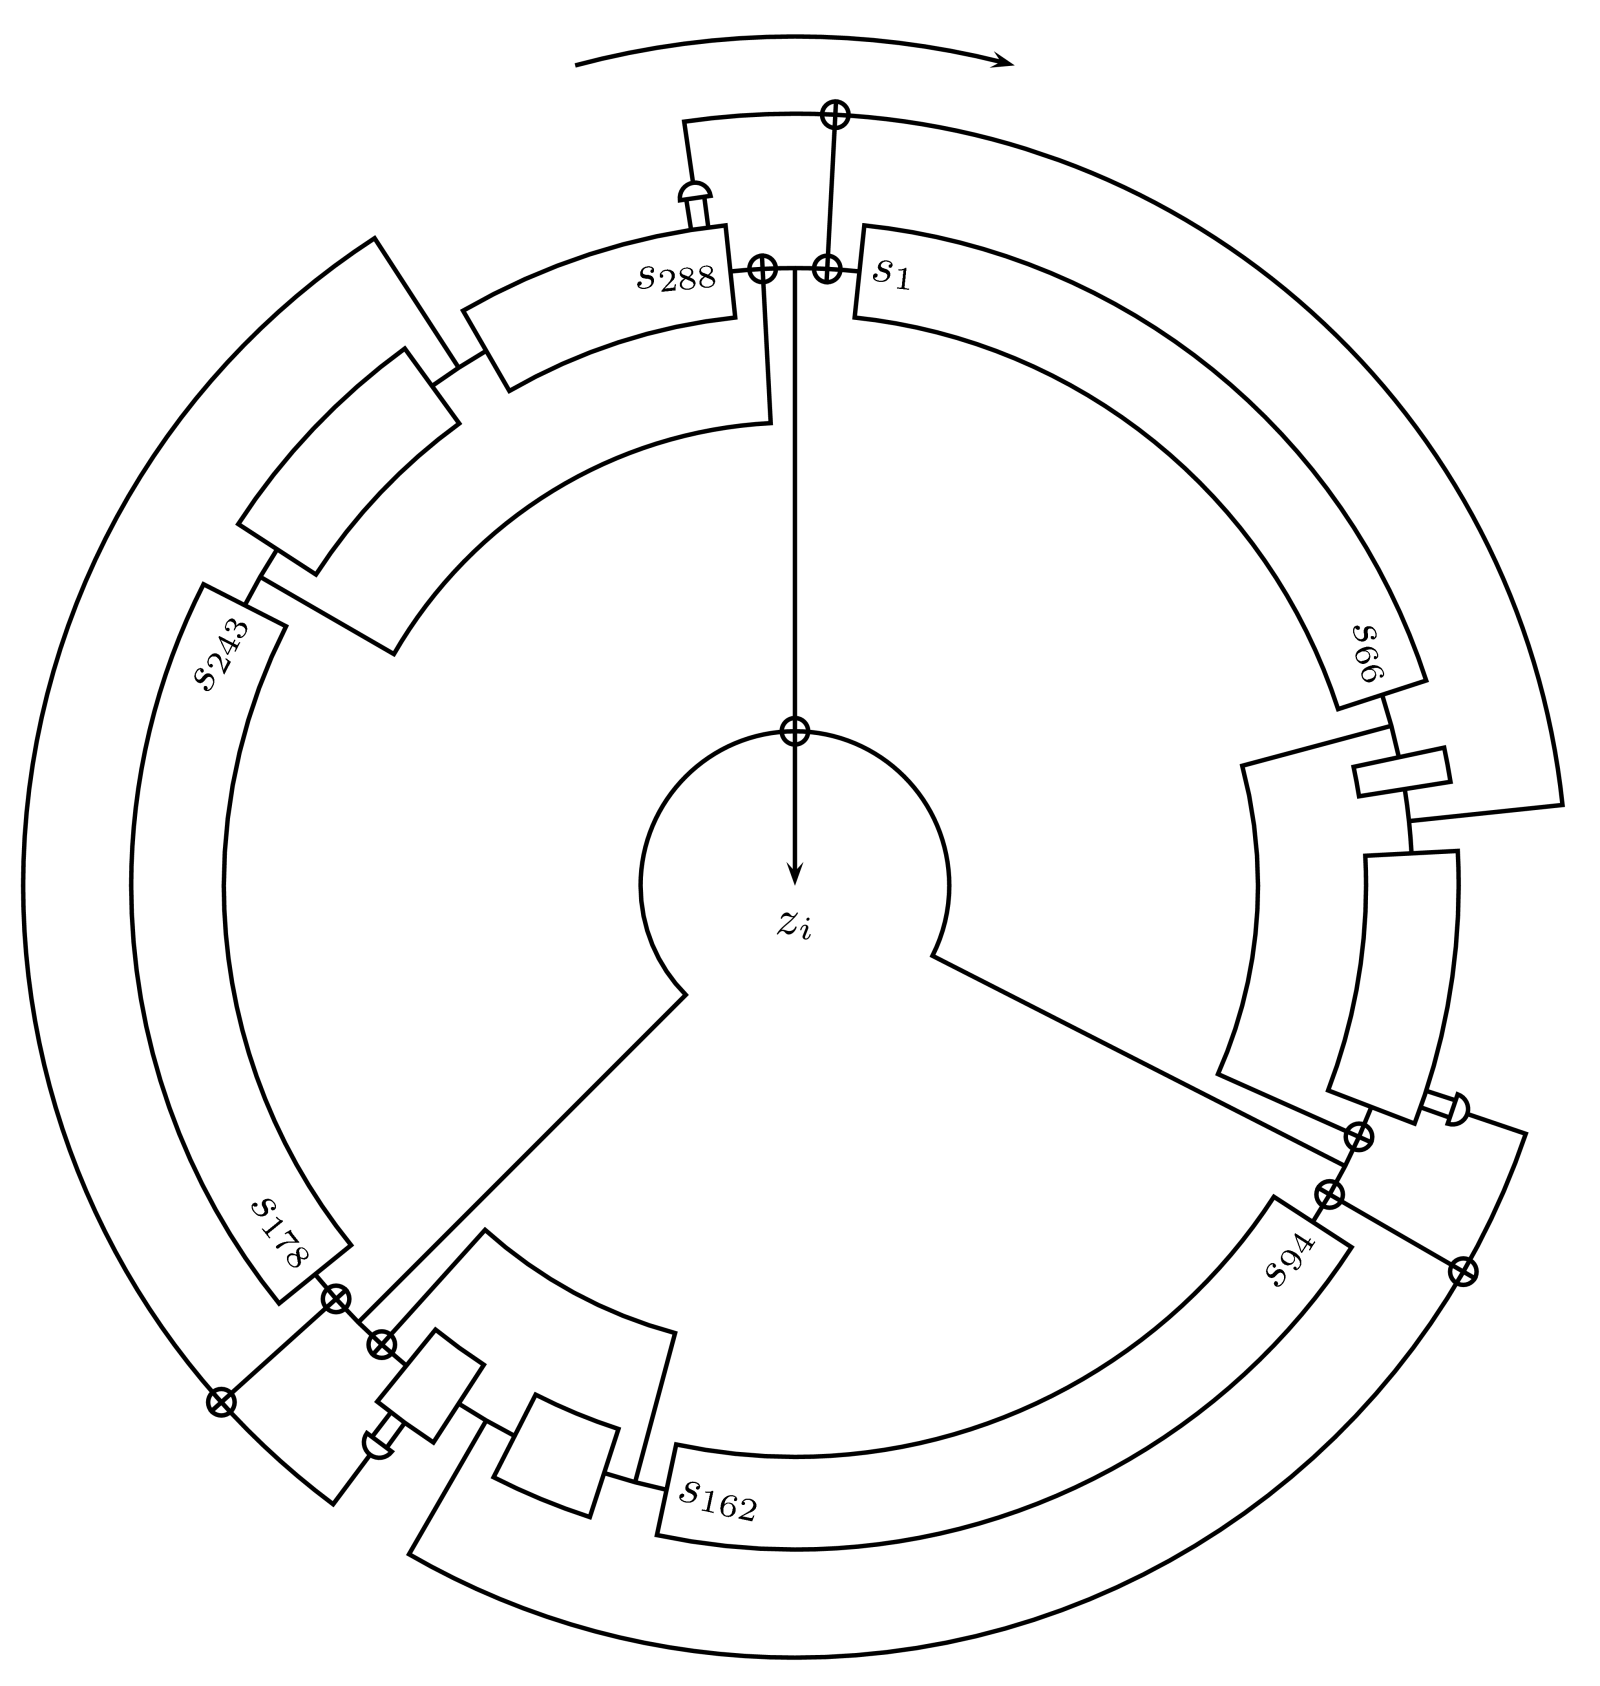
\includegraphics[scale=0.1]{screenshots/Trivium_(cipher).png}
	\caption{Structure of Trivium (Wikipedia)}
	\label{fig:}
\end{figure}
\begin{parag}{Bit Security and Consequences}
    The \important{cost of breaking}, the goal is to exploit a mathematical property or bug that can break the scheme much faster than $2^{\left|K\right|}$ attempts, which therefore \important{reduce the bit security}. As we can see the difficulty of those scheme is in the design of mathematically secure and subtly resistant primitives which has been found to be incredibly hard.
	\begin{subparag}{Best practice}
	    Use \important{well-vetted}, \important{peer-reviewed}, \important{standard algorithms and their implementation} (like AES, ChaCha20, SHA-3)
	\end{subparag}
\end{parag}





\section{Public Key Cryptography}

\begin{parag}{The Key Distribution Problem}
    As seen before, symmetric ciphers are fast, but require a pre-shared secret key. But a more fundamental question come first, if Eve can observe all conversation between Alice and Bob, how can they first agree on a secret key without having Eve to know?\\
	$ $\\
	The answer to that is public-key cryptography which allowed two parties who have never met to establish a secure channel. A famous example is Diffie-Hellman
\end{parag}
\begin{parag}{Diffie-Hellman Setup}
    Alice, Bob (and Eve) know a large public parameters: a prime number $p$ and a generator $g$
	\begin{subparag}{Alice Actions}
	    \begin{itemize}
	        \item Choose a \important{private} secret $a$
	        \item Compute the public value $A =  g^{a} \Mod p$
	        \item Sends $A$ to Bob
	    \end{itemize}
	\end{subparag}
	\begin{subparag}{Bob's Actions}
	    \begin{itemize}
	        \item Chooses a private secret $b$
	        \item Computes the Public Value $B = g^{b} \Mod p$
	        \item Sends $B$ to Alice
	    \end{itemize}
	\end{subparag}
	\begin{framedremark}
	Eve sees $A, B, g$ and $p$ but cannot find $a$ or $b$ due to the Discrete Log Problem, while it has a low complexity to compute g to the power b modulo p (with fast modular exponentiation algorithm, for example), there are no known fast (polynomial) algorithm to recover a from A and p (or b from B and p).
	\end{framedremark}
\end{parag}
\begin{parag}{The Shared Secret}
    Both Alice and Bob can compute a shared secret $K$
	\begin{align*} 
		K = B^{a} \Mod p &= \left(g^{b}\right)^{a} \Mod p\\
						 &= g^{ba} \Mod p\\
						 &= g^{ab} \Mod p\\
						 &= \left(g^{b}\right)^{a} \Mod p = A^{b} \Mod p
	\end{align*}
	Where but $B^{a} \Mod p$ and $A^{b} \Mod p$ are computable by Alice and Bob resp. However Eve cannot compute $K$ ,because she has neither $a$ nor $b$.
\end{parag}

\begin{parag}{Trapdoor Functions}
    This example of DF is one of the many examples of how to do public key cryptography to establish a shared secret (a shared key) to then do symmetric cryptography. They boil down to mathematical functions that are \important{easy to compute} in one direction but \important{hard} (high complexity) to do in the other direction. Those rely on underlying difficulty, for DH it is the \important{Discrete Logarithm Problem}.
\end{parag}
\begin{parag}{Beyond DH}
    There are other ways to set a shared secret (or even to directly communicate), all involve interesting mathematics.
	\begin{itemize}
	    \item \important{RSA}: Based on the factoring problem
	    \item \important{Elliptic Curve Cryptography (ECC)}: Can do Discrete Log on ECC, instead of on public-key crypto
	    \item \important{Post-Quantum Cryptography}: new primitives (like \important{Lattice Crypto}) to resist quantum computers.
	\end{itemize}
\end{parag}
\begin{parag}{Man In The Middle (MITM)}
    The classical version of Diffie-Hellman is vulnerable to active attack, as it only guarantees key agreement, but not authenticity (verifying who you are agreeing with). If for instance Eve intercepts $A$ from Alice and $B$ from Bob. Eve can impersonates : 
	\begin{itemize}
	    \item Eve sends $E_B$ to Alice. Alice compute $K_{AE}$
	    \item Eve Sends $E_A$ to Bob. Bob compute $K_{BE}$
	    \item Eve shares a key $K_{AE}$ with Alice and a separate key $K_{BE}$ with Bob.
	    \item She can read, modify and relay all communication.
	\end{itemize}
	Hence this implies a need for \important{trust} (authentication). DH solves the key distribution problem but create the identity verification one. The solution to this is that DH must be paired with a mechanism (like digital signature) to verify identity. The setup in this case requires a third party that needs to be trusted (a certificate authority) for public key ownership.
\end{parag}






















\subsection{Authenticity}
We have found a way to encrypt messages, meaning no one can see our messages from outside, but in the first place we have to make sure that our messages go to the right persons and vis versa, we need to be able to be sure that the message we have received is from the right person. Do to do, one need to define \important{authenticity}. 
\begin{definition}{(Authentication)}
	The process of verifying a claimed identity.
\end{definition}
\begin{parag}{Ways to prove who you are}
    Traditionally, we have a lot of methods in order to authenticate ourself :
	\begin{itemize}
	    \item \textbf{What you know}: password, secret key
	    \item \textbf{What you are}: biometrics
	    \item \textbf{What you have}: smart card, secure token
	\end{itemize}
	However now what can use many other ways to prove :
	\begin{itemize}
	    \item \textbf{Where you are}: location, IP address
	    \item \textbf{How you act} behavioural authentication
	    \item \textbf{Who you know}: social ties
	    \item $\vdots$
	\end{itemize}
	
	
\end{parag}

\begin{parag}{Public key cryptography}
    To go back on public key cryptography, the way it worked was that we needed a public key infrastructure which allowed us to expose our public keys to the world in order to communicate. To do so we need \important{digital signature}, \important{signing} and \important{verification}. The public key infrastructure needs to ensure authenticity. \\
	$ $\\
	Imagine now that Bob (secret key $SK$, public key $PK$) and Bob wants to communicate, he will send a message $M$ and also a \important{signing} defined as
	\begin{align*} 
		\text{Sign}_{SK}\left(M\right) = S 
	\end{align*}
	and send this back to Alice which she can verify using here own function $V_{PK}$
	\begin{align*} 
		V_{PK}\left(M, S\right) =  \checkmark
	\end{align*}
	\begin{center}
	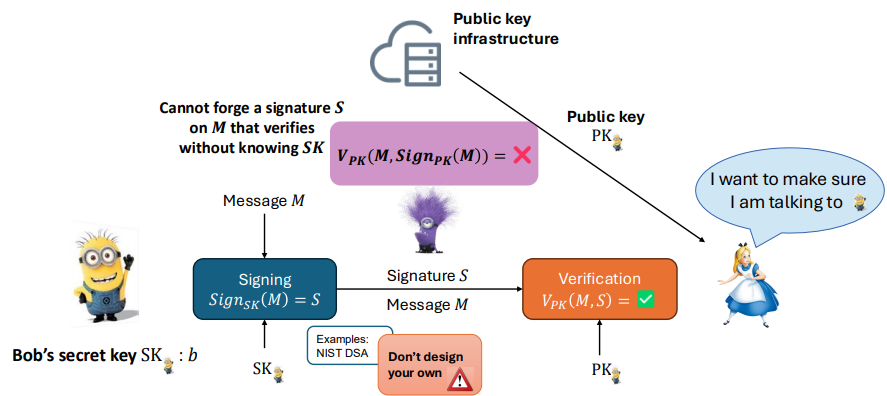
\includegraphics[scale=0.4]{screenshots/2026-10-15.png}
	\end{center}
\end{parag}
So how it works is the following 
\begin{itemize}
    \item Bob has a secret key. Using this key Bob performs a \important{digital signature} on the message.
    \item To verify a signature, Alice get Bob's public key from the repository and performs a verification function using the message, the signature, and Bob's public key. This function returns yes if the signature is valid, and no otherwise.
\end{itemize}
    To be secure, and provide integrity, Digital Signature algorithms need to be such that it is not possible to create a Signature for a message that will verify under a given public key, unless you have the corresponding secret key. Under these properties, a digital signature enable Alice to know that she is talking to Bob: only Bob, that knows the secret key, could have created the signature.

\begin{parag}{Digital signatures}
    Digital signatures are computationally costly compared with most symmetric key algorithms of equivalent security, what this means concretely is that signing and encrypting is \important{slow} (not having to pre-share a key comes at a cost).\\
	$ $\\
	Naively, this gives us a big issue, having long message implies that the signing and verification will take a very long time and will be not practical, if you remember CS-200, you may remember the way to solve that issue :
\end{parag}
\subsection{Hash Functions}
\label{par:Hash functions}
Hence, let us define three security properties that a hash function require
\begin{itemize}
    \item \textbf{Pre-image resistance}: Given $H =  h\left(M\right)$, it should be difficult to find $M$
    \item \textbf{Second Pre-image resistance}: Given $M$, difficult to find $M' \neq M$ such that $h\left(M'\right) = h\left(M\right)$
    \item \textbf{Collision Resistance}: difficult to find any $M, M'$ such that $h\left(M\right) =  h\left(M'\right)$
    \item \textbf{Deterministic}: Given $M$ a hash function $H$ will always output the same string $h =  H\left(M\right)$
\end{itemize}
Cryptographic hash functions are designed to be fast and efficient to compute, and they have several important properties that make them valuable in various applications.

\begin{figure}[h!]
\centering
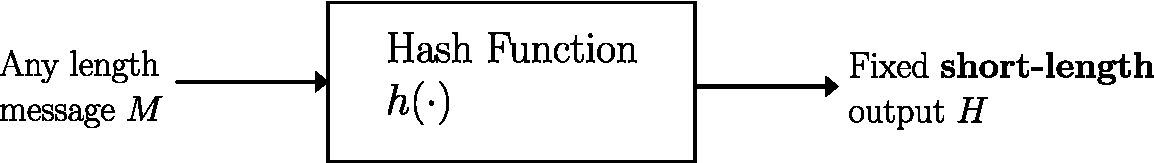
\includegraphics[width=0.8\textwidth]{figure/2026-10-15.pdf}
\caption{A beautiful diagram of a hash function (right?)}
\end{figure}

As always, one should never design those themselves and should use already existing hash functions 
\begin{itemize}
    \item MD5 (1991): 128 bits hash --- insecure
    \item SHA0, SHA1: 160 bits --- insecure
    \item SHA-2 (224/256 /384/512) --- Ok but slow
    \item SHA-3 (224/256 /384/512)
\end{itemize}
The use cases of hash function are vast, in order to support digital signatures, build HMAC, password storage, file integrety, secure commitments, secure logging, blockchains, ...


\begin{parag}{Digital signatures on hash functions}
	So now instead of having a digital signature on the whole message (which can be enormous), one can sign using the \important{hash} of the message. Meaning that instead of having $\text{Sign}_{SK}\left(M\right) =  S$, we will replace $M$ by $H = h\left(M\right)$. Alice on the other side will receive both the signature and the message and also need to compute the hash of the message on her side in order to apply the verification.\\
	$ $\\
    So how it works is the following: only Bob has his secret key $SK$, so only Bob can produce a signature $S$ that verifies under his public key $PK$. When Alice checks $V_{PJ}\left(h\left(M\right), S\right) = \checkmark$, she learns two things:
	\begin{itemize}
	    \item \important{origin}: the signature was made by whoever holds Bob's $SK$, which should be Bob
	    \item \important{Integrity}: $M$ wasn't modified. Changing $M$ changes $h\left(M\right)$, so the old signature no longer verified it.
	\end{itemize}
\end{parag}
\begin{framedremark}
Note that Preimage resistance is not needed here, as the message $m$ is already sent in public.
\end{framedremark}

\begin{parag}{All together}
    Now let us have both the encryption of the message and the signature so that we ensure, privacy and authentication. This implies that each users have \important{two pairs} of keys (2 $\times$ secret key, 2 $\times$ public key). In that case \important{confidentiality} is ensured as before with the ciphertext
	\begin{align*} 
		C = E_{PK}\left(M\right)
	\end{align*}
	and the decryption computed as 
	\begin{align*} 
	 	D_{SK}\left(c\right)
	\end{align*}
	$ $\\
	The authentication on the other hand is using the other pair of keys with
	\begin{align*} 
		 V_{PK}\left(M, S\right) = \checkmark \text{ with } S = \text{Sign}_{SK}\left(M\right)
	\end{align*}
	\begin{center}
	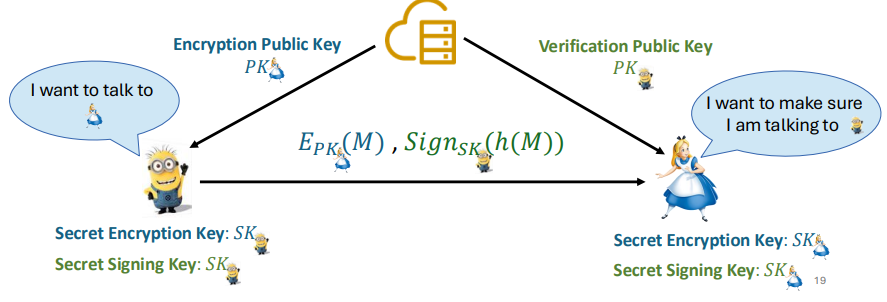
\includegraphics[scale=0.4]{screenshots/2026-10-15_1.png}
	\end{center}
\end{parag}


\subsection{Integrity}

Now we have again another problem \important{Integrity} 
\begin{definition}{(Integrity)}
information cannot be \important{modified} by unauthorized parties
\end{definition}

What this means is that if Bob sends '\textit{Banana}' he can be sure that Alice will receive '\textit{Banana}'.
\begin{parag}{Message integrity through digital signatures}
    As seen before in asymmetric cryptography, we have already seen a way to solve the integrity problem: digital signatures. Those provide 
	\begin{itemize}
	    \item Sender authenticity: since no party than the sender can create a valid signature for a message, the server can verify that the identity of the sender. No adversary can produce a valid signaature to the public key of the sender and therefore cannot impersonate the sender
	    \item Integrity of the message: Since no party than the sender can create a valid signature for a message, no adversary can modify the message without being detected (if they modify the message, the signature would not be valid)
	    \item Non-repudiation: Since no party than the sender can create a valid signature for a message, if a message has a valid signature, the sender cannot claim they did not sign it (no-one else can produce such signature).
	\end{itemize}
	However what this gives is that the signature $S$ only verified if message $M$ has not been modified
\end{parag}

\subsubsection{Integrity for Symmetric Cryptography}
    As in the asymmetric cryptography schemes, symmetric ones should also not have to suffer through integrity! Let us take the example of Block cipher,  meaning the message is sent by block of fixed size, typically 128/256 bits. What this implies is that in order to send a message of size greater than a block, we require iteration, which implies that we need to create some sort of mode operation:

\begin{parag}{Mode 1: Electronic Code Book (ECB)}
	Straightforward scheme: encrypt and decrypt single blocks. So we work as a '\textit{stream}' with each $M_i$ being encrypted with $E_K\left(\cdot \right) \to C_i$. For which we can then reconstruct the message as 
	\begin{align*} 
		M = M_1M_2M_3M_4\cdots 
	\end{align*}
	Which each block with the same size as the key. However we have a big issue here imagine that $M_i =  M_j$, what this gives is 
	\begin{align*} 
		M_i \to E_K\left(\cdot \right) \to C_i \\
		\underbrace{M_j}_{= M_i} \to E_K\left(\cdot \right) \to C_i
	\end{align*}
	\begin{center}
	    if $M_i = M_j$ then $C_i =  C_j$
	\end{center}
	which implies that the attacker learns something about the plaintext without breaking the cipher. Confidentiality means the ciphertext should reveal nothing about the message except its length. With ECB, it reveals which blocks are equal and that alone is often enough to learn a lot.
	
\end{parag}
\begin{parag}{Mode 2: Cipher Block Chaining (CBC)}
    The idea in this technique is to add some "\textit{noise}" in the encryption by block in order to '\textit{hide}' the equals blocks. We create an Initialization Vector (IV) which is a random block and the encrypt using the following rule 
	\begin{align*} 
		C_0 &=  IV\\
		C &= E_K\left(M_i \oplus C_{i-1}\right)
	\end{align*}
	\begin{center}
	\includesvg[scale=0.7]{figures/CBC_encryption.svg}
	\end{center}
	Where each block cipher encryption is $E_K\left(\cdot \right)$.
	\begin{subparag}{Remark}
	    Note that every time a block is encrypted, by the properties of the block cipher, the ciphertext is random. Because the IV and/or the plaintext changes every time, this random value is different every time. Thus, when XORed with the next plaintext it creates a random string. If the IV changes, this is similar to a one-block one-time pad, but if one reuses the IV for the same plaintext and key, this value will be repeated.
	\end{subparag}
\end{parag}
\begin{parag}{Decryption of CBC}
    In order to decrypt messages all we need to do is work the other way around. Recall that $C_0 =  IV$ and that $C_1 = E_K\left(M_1 \oplus IV\right)$. Decrypting it gives $D_K\left(C_1\right) = M_1 \oplus IV$ which means that we can recover $M_1$ as $M_1 =  M_1 \oplus IV \oplus IV$. Hence, given $C_i =  E_K\left(M_i \oplus C_{i-1}\right)$, Alice can decrypt it as $D_K\left(C_i\right) = M_i \oplus C_{i-1}$, by applying $\oplus C_{i-1}$ to it.
	\begin{align*} 
		M_i &= D_K\left(C_i\right) \oplus C_{i-1} \\
		&= M_i \oplus C_{i-1} \oplus C_{i-1}\\
		&= M_i
	\end{align*}
	However this raises some questions: what if $IV$ is incorrect? Is the full decryption wrong? Can you decrypt a block alone? What do you need?\\
	$ $\\
	If the IV is incorrect, only the first block is corrupted, Recall that the rest only depend on the ciphertext. Note also that blocks cannot be decrypted without having the previous ciphertext!
\end{parag}


\begin{parag}{Mode 3: Counter Mode (CTR)}
    The idea here it to use increasing nonce to add randomness without dependencies between block. What this means is that the CTR encryption is defined as 
	\begin{align*} 
		C_i =  E_K\left(\text{Nonce} + i\right) \oplus M_i 
	\end{align*}
	\begin{center}
	
\includegraphics[scale=0.17]{screenshots/CTR_encryption.png}
	\end{center}
	Now the question is how do we decrypt this cipher? Well if you think about it:
	\begin{align*} 
		M_i = E_K\left(\text{Nonce} + i\right) \oplus C_i 
	\end{align*}
	right? Let us see if this is true 
	\begin{align*} 
		E_K\left(\text{Nonce} + i\right) \oplus C_i &= E_K\left(\text{Nonce} + i\right) \oplus E_K\left(\text{Nonce} + i\right) \oplus M_i\\
													&= M_i
	\end{align*}
\end{parag}
\begin{parag}{Block Ciphers}
    \begin{subparag}{Strengths}
        \begin{itemize}
            \item \textbf{High diffusion}: information from one plaintext symbol is diffused into several ciphertext symbols
            \item \textbf{Immunity to tampering}: difficult to insert symbols without detection
        \end{itemize}
    \end{subparag}
	\begin{subparag}{Weaknesses}
	    \begin{itemize}
	        \item \textbf{Slow}: an entire block must be accumulated before encryption/ decryption can begin
	        \item \textbf{Error propagation}: in some modes of operation errors affect several bits/blocks
	    \end{itemize}
	    
	\end{subparag}
\end{parag}

\paragraph{Summary}%
\label{par:Summary}

\begin{itemize}
    \item \textbf{Electronic Code Book (ECB)}: Directly encrypt and decrypt single blocks. Large information leakage due to lack of randomness across block's encryption
    \item \textbf{Cipher Block Chaining (CBC)}: Avoids ECB problems by using previous blocks to add randomness to every encryption. Propagates errors and prevents single-block decryption
    \item \textbf{Counter mode (CTR)}: Uses an increasing '\textit{nonce}' to introduce randomness across block's encryptions. Enable parallel encryption and decryption.
\end{itemize}

\paragraph{What about integrity?}%
\label{par:What about integrity?}
As in the asymmetric case, let us see how to ensure integrity for symmetric encryption. To do so we'll use \important{message authentication code} (\important{MAC}).
\begin{center}
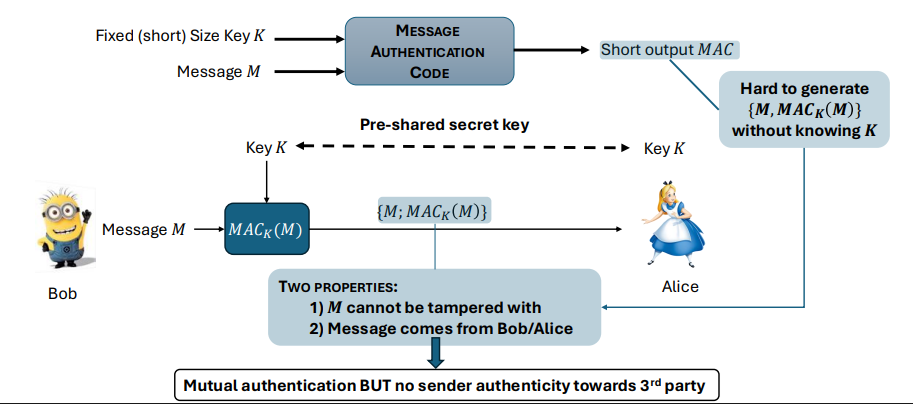
\includegraphics[scale=0.4]{screenshots/2026-10-15_2.png}
\end{center}
A MAC is like a hash function with a \important{key}. It takes a shared secret $K$ and a message $M$ and outputs a short tag $MAC_K\left(M\right)$. Alice computes $T =  MAC_K\left(M\right)$ and sends $\left\{M, T\right\}$. \\
$ $\\
Bob then receives $\left\{M, T\right\}$ and recomputes $MAC_K\left(M\right)$ himself using $K$, and checks whether it equals $T$.\\
$ $\\
But first let us be a bit more '\textit{formal}' about the defintion of our MAC. A message authentication code receives two inputs:
\begin{itemize}
    \item A small key that must be kept secret
    \item The message who integrity needs to be secured
\end{itemize}
The MAC algorithm outputs a short string that helps Alice to verify the integrity of the message sent by Bob.\\
$ $\\
The key property of the MAC is that it is very difficult to produce a pair [message; $MAC\left(k, \text{message}\right)$] without knowing the key.\\
$ $\\

This is the symmetric counterpart of a signature check. The difference is that Bob can't merely verify: he recomputes the exact same value, because he hols the same key. The integrity here comes from the fact that if Eve changes $M$, the tag no longer matches and she can't compute a new one without $K$. The authenticity on the other hand comes from that only someone who knows $K$ could have made the tag, so it came from Alice or Bob.
\begin{parag}{Repudiation}
    Now imagine an exchange between Alice and Bob with Charlie being a third party observes. Even though Alice and Bob know they are talking to each other (only any party with knowledge of $K$ could have produce a valid MAC, message pair, they both could have produced the message.)\\
	So the message can be repudiated which means both A and B can claim it was the other who wrote the message.
\end{parag}

\begin{parag}{Example MAC: CBC-MAC}
    Let us see how to turn a block cipher into a mac. To do so CBC MAC defines the following encryption methods 
	\begin{align*} 
		C_0 &= 0 [\text{ any fixed }IV] \\
		C_i &= E_K\left(M_i \oplus C_{i-1}\right)\\
		MAC_K\left(M_1 \ldots M_x\right) &=  C_n
	\end{align*}
	The difference here with CBC encryption is that CBC-MAC is deterministic, also only the output of CBC-MAC is the last block.
	\begin{subparag}{Remark}
	    Remark that CBC can be turned into a MAC by:\\
		$ $\\
		Fix $IV$ (e.g. 0) and then do CBC. The MAC is the output of the last encryption block: one could have only gotten there for one message and one key. Note that the last block cannot be used to recover anything about the message: it looks random (as it is the output of a block cipher)
	\end{subparag}
	\begin{subparag}{Limitation}
		The encryption scheme is only secure if the length of the message $M$ is known.
	\end{subparag}
	\begin{center}
	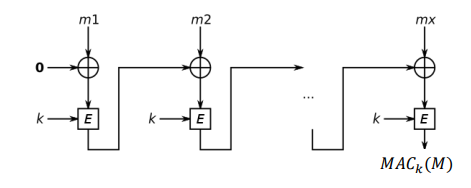
\includegraphics[scale=0.5]{screenshots/2026-10-15_3.png}
	\end{center}
\end{parag}

\paragraph{And all together now ...}%
\label{par:And all together now ...}

    \begin{parag}{Encrypt and MAC}
        \begin{itemize}
			\item $\times$ No integrity on the ciphertext $\to$ Cipher can be attacked which therefore mean that we need to decrypt to know if the ciphertext is valid
			\item \checkmark integrity of the plaintext can be verified
			\item $\times$ May reveal information about the plaintext $\to$ repeated messages, recall the $IV$ of the MAX is fixed (can be solved with a counter)
        \end{itemize}
        \begin{center}
        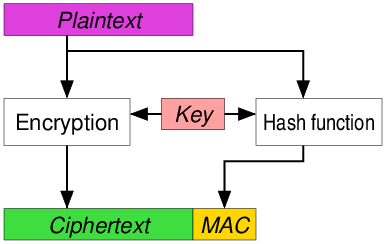
\includegraphics[scale=0.4]{screenshots/Authenticated_Encryption_EaM.png}
        \end{center}
    \end{parag}
	\begin{parag}{MAC then encrypt}
	    \begin{itemize}
	        \item $\times$ No integrity of ciphertext (in theory) it is possible to change ciphertext and have a valid MAC
	        \item \checkmark Integrity of the plaintext can be verified
	        \item \checkmark No information on the plaintext either, since it is encrypted
	    \end{itemize}
	    \begin{center}
	    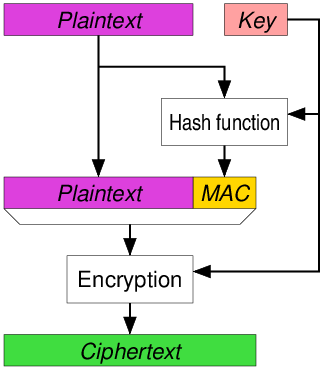
\includegraphics[scale=0.4]{screenshots/Authenticated_Encryption_MtE.png}
	    \end{center}
	\end{parag}
	\begin{parag}{Encrypt then MAC}
	    \begin{itemize}
	        \item \checkmark Integrity of ciphertext $\to$ ensures you only read valid massages! Cipher cannot be attacked!
	        \item \checkmark Integrity of the plaintext can be verified
	        \item \checkmark No information on the plaintext either, since it is encrypted
	    \end{itemize}
	    \begin{center}
	    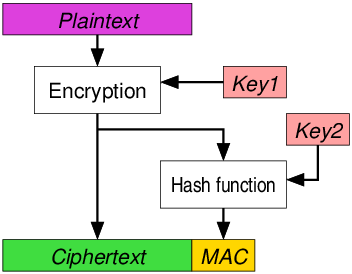
\includegraphics[scale=0.4]{screenshots/Authenticated_Encryption_EtM.png}
	    \end{center}
	\end{parag}
















\end{document}
